%%%%%%%%%%%%%%%%%%%%%%%%%%%%%%%%%%%%%%%%%%%%%%%%%%%%%%%%%%
\section{\label{sec:Technicalities}Technicalities}
%%%%%%%%%%%%%%%%%%%%%%%%%%%%%%%%%%%%%%%%%%%%%%%%%%%%%%%%%%

%%%%%%%%%%%%%%%%%%%%%%%%%%%%%%%%%%%%%%%%%%%%%%%%%%%%%%%%%%
\subsection{\label{sec:Technicalities:BoltzmannEquation}The Boltzmann equation and its solution}
%%%%%%%%%%%%%%%%%%%%%%%%%%%%%%%%%%%%%%%%%%%%%%%%%%%%%%%%%%

In order to compute the distribution functions of the scalar and the sterile neutrino, we employ the Boltzmann equation, $\hat{L}[f]=\mathcal{C}[f]$, where $f$ is the distribution function we want to determine, $\hat{L} = \frac{\partial}{\partial t} - H p \frac{\partial}{\partial p}$ (with the Hubble function $H$) is the Liouville operator in a homogeneous and isotropic Friedman-Robertson-Walker universe, and $\mathcal{C}$ contains the collision terms describing interactions of the particles.\footnote{This is already an approximation in itself because, by using the Boltzmann equation -- which is a classical equation -- we do neglect quantum corrections. To include those, Kadanoff-Baym equations must be used, which are way more difficult to solve. The error caused by the approximation we make here is of $\mathcal{O}(10\%)$ in the abundance~\cite{Hamaguchi:2011jy}.} In our case, we actually need to solve two coupled Boltzmann equations, for the two distribution functions $f_N$ and $f_S$ of the sterile neutrino $N$ and the scalar $S$, respectively:
\begin{eqnarray}
 \hat{L}f_S &=& \mathcal{C}^S \label{eq:Boltzmann_Scalar}\ \ \ {\rm and}\\
 \hat{L} f_N &=& \mathcal{C}^N. \label{eq:Boltzmann_Neutrino}
\end{eqnarray}
The collision terms are themselves sums of several individual terms which encode the details of the respective processes as well as information on whether they contribute to production or depletion of the species under consideration. Depending on the regime, various diagrams listed in Tab.~\ref{tab:RegimesFeynman} can contribute to the production of scalars and hence, ultimately sterile neutrinos. Explicitly, the scalar collision term $\mathcal{C}^S$ consists of the following:
\begin{itemize}
\item Regime~I ($T>T_\text{EWPT}$):
\begin{align}\label{eq:ct_scalar_above_pt}
\mathcal{C}^S_\text{I} = \mathcal{C}^S_{\phi\phi \leftrightarrow SS} + \mathcal{C}^S_{S \rightarrow NN}.
\end{align}
\item Regime~II ($T<T_\text{EWPT}$  and  $m_S> m_h/2$):
\begin{align}\label{eq:ct_scalar_below_pt_large_m}
\mathcal{C}^S_\text{II} = \mathcal{C}^S_{hh \leftrightarrow SS} + \mathcal{C}^S_{t\bar{t} \leftrightarrow SS} + \mathcal{C}^S_{W^+W^- \leftrightarrow SS} + \mathcal{C}^S_{ZZ \leftrightarrow SS} + \mathcal{C}^S_{S \rightarrow NN}.
\end{align}
\item Regime~III ($T<T_\text{EWPT}$ and  $m_S < m_h/2$):
\begin{align}\label{eq:ct_scalar_below_pt_small_m}
\mathcal{C}^S_\text{III} =\mathcal{C}^S_\text{II} + \mathcal{C}^S_{h \leftrightarrow SS}.
\end{align}
\end{itemize}
The labels should be quite intuitive. For example, in regime~I, the term $\mathcal{C}^S_{\phi\phi \leftrightarrow SS}$ encodes both the annihilation of two Higgs doublets $\Phi$ into two scalars $S$ and vice versa, with opposite signs for the two cases. On the other hand, $\mathcal{C}^S_{S \rightarrow NN}$ will always come with a negative sign, since it only describes the decay of the scalar into sterile neutrinos. Similarly, the only difference between regimes~II and~III is the appearance of the Higgs decays into two scalars, $\mathcal{C}^S_{h \leftrightarrow SS}$, for sufficiently small scalar masses. 

The sterile neutrino collision term is comparatively simple, and it is given by:
\begin{align}
 \mathcal{C}^N = \mathcal{C}^N_{S \rightarrow NN},
 \label{eq:ct_sterile_neurtrino}
\end{align}
but in this case with a positive sign as it creates sterile neutrinos. Here we neglected the inverse decay, i.e.\ the process $NN \rightarrow S$, because the sterile neutrino is a FIMP, such that its abundance is always far below its would-be equilibrium abundance for large enough temperatures $T$. Hence the process $NN \rightarrow S$ is suppressed by the small number of sterile neutrinos present in the Universe.

Note that the collision terms will in general depend on the distribution functions $f_i$ of \emph{all} particle species $i$. However, as argued, we only need to compute the distributions $f_S$ and $f_N$, since all SM species can be assumed to be in thermal equilibrium such that their distributions are well approximated by simple Boltzmann factors.\footnote{As already anticipated, this is a non-trivial assumption for the SM Higgs boson. We have shown explicitly that the Higgs only freezes out at relatively small temperatures, $T\sim 3$~GeV, which is due to its decay into SM particles keeping it in equilibrium for a longer time than naively expected for a WIMP-like particle. This also provides an a posteriori justification of the assumption made by Adulpravitchai and Schmidt in Ref.~\cite{Adulpravitchai:2014xna}. See App.~\ref{app:B:Higgs-FO} for details.} To anticipate one particular example collision term, we quote from Eq.~\eqref{eq:CT_N_App} the one describing the production of sterile neutrinos of momentum $p$ at temperature $T$ by the decaying scalars,
\begin{align}
 \mathcal{C}^N_{S \rightarrow NN}[f_S](p , T) = \frac{y^2 m_S^2}{16 \pi p^2}\int\limits_{p'_\text{min,N}}^\infty \mathrm{d}p'\ \frac{p' \; f_S(p',T)}{\sqrt{m_S^2 + p'^2}},
 \label{eq:CT_N}
\end{align}
where the lower boundary of the integral over scalar momenta $p'$ is given by $p'_\text{min,N} = \left| p - \frac{m_S^2}{4 p} \right|$. This term is indeed positive, since it produces sterile neutrinos. As expected, this equation contains the distribution function $f_S$ of the scalar at temperature $T$, making it explicit that Eqs.~\eqref{eq:Boltzmann_Scalar} and~\eqref{eq:Boltzmann_Neutrino} are coupled and have to be solved as a system of equations. For a detailed discussion of all collision terms we refer the reader to App.~\ref{app:coll_terms}.





%%%%%%%%%%%%%%%%%%%%%%%%%%%%%%%%%%%%%%%%%%%%%%%%%%%%%%%%%%
\subsubsection{\label{sec:Technicalities:BoltzmannEquation-solution}How to crack a coupled system of non-linear partial integro-differential equations in two variables}
%%%%%%%%%%%%%%%%%%%%%%%%%%%%%%%%%%%%%%%%%%%%%%%%%%%%%%%%%%

Glancing at the explicit forms of the collision terms in App.~\ref{app:coll_terms}, we can see that the task of computing sterile neutrino production from scalar decay is a highly non-trivial one: it necessitates the solution of a coupled system of partial integro-differential equations in two variables. In an abstract, yet intuitive manner, the system of equations we have to solve turns out to have the following form:\footnote{Note that, at this point, we could also have taken an alternative route. The part of the integral that only contains Boltzmann distributions does \emph{not} depend on $f_S$ and could hence, in principle, be integrated numerically. This would result in a numerical function of the form $\mathcal{F}(p,T)$ on the right-hand side of the first Eq.~\eqref{eq:Boltzmann_system}. However, this strategy would have at least two drawbacks: 1.) First, the structure of the equation would be much less clear, since several crucial dependencies would just be ``hidden'' inside a numerical function $\mathcal{F}(p,T)$. 2.) Furthermore, this procedure would ultimately force us to subtract two numerically computed integrals from each other, which is numerically less accurate than first computing the difference of the integrand functions before evaluating the integral over their difference. We thus stick to the strategy outlined in the main text.} 
\begin{eqnarray}
 \hat{L} f_S\left(p,T\right) &=& \mathcal{D}\left(p,T\right) f_S\left(p,T\right) + \int\limits_{0}^{\infty}{\diffd p'\mathcal{K}^{S}\left(p,p',T\right)\left[f_S\left(p,T\right) f_S\left(p',T\right) - f_S^{\mathrm{eq}}\left(p,T\right) f_S^{\mathrm{eq}}\left(p',T\right) \right]}  \,, \nonumber\\
 \hat{L} f_N\left(p,T\right) &=& \int\limits_{0}^{\infty}{\diffd p'\mathcal{K}^N\left(p,p',T\right) f_S\left(p',T\right)} \,,  \label{eq:Boltzmann_system}
\end{eqnarray}
where $\mathcal{K}^{S/N}$ and $\mathcal{D}$ are known functions directly related to the collision terms $\mathcal{C}$, and $f_i^{\mathrm{eq}}$ denotes the (possibly hypothetical, in case the interactions are too feeble) equilibrium distribution of particle $i$.

The question is now how to tackle such a problem. Before starting the computation we note that, while the sterile neutrino distribution function $f_N$ does depend on the distribution function $f_S$ of the scalar, the converse is not true. The reason is that, as we had argued, we can neglect any inverse processes involving sterile neutrinos. This already yields to a considerable simplification, allowing us to solve the first Eq.~\eqref{eq:Boltzmann_system} independently and to then insert the result obtained into the second equation. However, even then, we are still left with a non-linear partial integro-differential equation in $f_S$ which is highly non-trivial to solve numerically (and impossible to solve analytically). We will thus need to play some tricks, in order to tame this equation.

The first step is to perform a transformation of variables, $(t,p) \to (r,\xi)$, such that the left-hand side of the first Eq.~\eqref{eq:Boltzmann_system} only involves a derivative with respect to a single variable. As shown in App.~\ref{app:transf_variables}, this is possible for $r=f(t)$ being an arbitrary function $f$ independent of the scalar momentum $p$, and $\xi(p,t) = g \left( \frac{a(t)}{a(t_0)} p \right)$ simultaneously being an arbitrary function $g$ of a specific combination of time $t$ and momentum $p$, which involves the scale factor $a(t)$ and an arbitrary reference time $t_0$. Thus, in fact, there exists a whole family of functions $f$ and $g$ which would simplify our complicated equation, however, choosing them in a smart manner may even lead to further simplifications. In our view, the following choice of variables is particularly convenient:\footnote{We exploit the one-to-one correspondence between cosmic time $t$ and plasma temperature $T$.}
\begin{align}\nonumber\label{eq:xi_and_r_definition}
r &= \frac{m_0}{T},\\
\xi &= \frac{1}{T_0}\frac{a(t)}{a(t(T_0))} \; p = \left( \frac{g_{s}(T_0)}{g_{s}(T)} \right)^{1/3}\;\frac{p}{T},
\end{align}
where $g_s(T)$ is the number of effective entropy degrees of freedom (for which we have used the numerical fit developed in Ref.~\cite{Wantz:2009it}). The arbitrary reference mass $m_0$ and temperature $T_0$ have been chosen by us to both equal the Higgs mass, $m_0 = T_0 = m_h$, which will later prevent us from working with extremely small or large numbers in our numerical computation. This choice of variables indeed implies certain simplifications, e.g., the Liouville operator now reads:
\begin{align}
\hat{L} = \frac{\partial r}{\partial t}\frac{\partial}{\partial r}= r H\left(r\right) \left( \frac{T g_s'}{3 g_s} + 1 \right)^{-1}\frac{\partial}{\partial r},\label{eq:liouville_final_form}
\end{align}
where $'$ denotes a derivative with respect to the temperature $T$. 

A valid interpretation of the new variables is to view $r$ as ``time'' variable and $\xi$ as ``momentum'' variable. Indeed, $r$ increases as the temperature decreases, just as the cosmic time $t$, so it can really be thought of as a rescaled or stretched time. In turn, $\xi$ can be thought of as something like a comoving rescaled momentum. Alternatively, one could think of it as a rescaled momentum that is red- or blue-shifted with respect to the reference temperature $T_0$. Indeed, the big advantage of the variable $\xi$ is that the distributions remain constant in time $r$ as soon as the production of particles is finished. For example, if the scalar $S$ was stable, its distribution for late time would be given by $f_S(\xi,r) \equiv f_S(\xi, r_\text{prod}),~~~\forall r \geq r_\text{prod}$, where $r_\text{prod}$ marks the time when no $S$-particles are produced anymore (e.g.\ the freeze-out time in case $S$ was a stable WIMP). This effect translates into the sterile neutrino distribution, i.e., $f_N$ will also be constant in $r$ once the scalar decays cease to be efficient. All redshifts of the momenta are automatically included in the definition of $\xi$.

The resulting form of the Boltzmann equations used in our implementation is
\begin{align}
 \frac{\partial f_i}{\partial r}( \xi, r ) = \frac{1}{r H(r)} \left( 1 - \frac{r }{3} \frac{\partial}{\partial r} \ln [g_s(r)] \right) \mathcal{C}^i[f_i,f_{j\neq i}],
 \label{eq:boltz}
\end{align}
where $i=S,N$. Indeed, we have by our substitution transformed the partial differential equation in two variables into an equation containing a differential with respect to one variable only. Of course, the collision terms in their general form of \Equref{eq:Boltzmann_system} have to be transformed according to this change of variables. Note that this general form can be written down for both the scalar and the sterile neutrino, but it is only necessary for the former, as the sterile neutrino evolution equation is comparatively simple once $f_S$ is known. We will therefore concentrate on the case $i=S$ in the following.

Still, the main issue remains: the collision term is nonlinear in $f_S$, and it furthermore includes an integral over $\xi$, which renders this equation to be of a partial integro-differential type, which are very difficult to solve. While several strategies for certain types of integro-differential equations (such as the Volterra-type) are available in the literature, the equation under consideration turns out not to be of any such type, so that we have to find a dedicated workaround. We apply a trick to get at least an (arbitrarily good) approximation by discretising the equations and substituting the integral over $\xi'$ by a finite sum over $M$ discrete momentum values $\xi_i,\, i\in\{1,...,M\}$. This transforms the original non-linear integro-differential equation~\eqref{eq:boltz} into a system of coupled non-linear ordinary differential equations for the different modes $f_S^i\left(r\right)$:
\begin{align}
 \dd{r} f_S^i\left(r\right) = \tilde{\mathcal{D}}^i\left(T\right) f_S^i\left(r\right) 
 + \sum\limits_{j=1,...,M}^{}{\tilde{\mathcal{K}}^{ij}\left(r\right)} \left[f_S^i\left(r\right)f_S^j\left(r\right) - f_S^{i,\mathrm{eq}}\left(r\right)f_S^{j,\mathrm{eq}}\left(r\right)  \right], \quad \forall i \in\{1,\dots,M \}.
\end{align}
Note that the integral results in a ``non-local'' coupling, since it couples any mode $f_S^i$ not only to some ``neighbouring'' modes, but to \emph{all} modes instead.

Finally, we have to numerically solve the resulting system of differential equations. This step involves one more difficulty, since the most simple strategies (such as the Runge-Kutta method) fail for large parts of the parameter space due to the stiffness of the system. Another more technical issue is that packages such as \textsc{Mathematica} natively employ list-based algorithms, while matrix-based ones are much more appropriate for the equations under consideration. We have thus found it more convenient to use the built-in \textsc{Matlab} solver \textit{ode15s}~\cite{Matlab:ode15s:reference1,Matlab:ode15s:reference2},  which is particularly efficient when dealing with stiff problems. Nonetheless, one should try to tweak any solver algorithm to take advantage of our a-priori knowledge that a distribution function must never attain negative values.
This way, we have been able to solve the equations for the scalar distribution functions $f_S$ efficiently. The resulting numerical functions can then be inserted into Eq.~\eqref{eq:boltz} for $i=N$ or, alternatively, one can use the ``master formula'' as given in Eq.~(16) of Ref.~\cite{Merle:2015oja}, once the variables are transformed according to Eqs.~\eqref{eq:xi_and_r_definition}.

Obtaining the functions $f_N (r,\xi)$ was the goal we wanted to reach. These distribution functions form the basis to compute all properties of the DM species for a given point in the parameter space, see Ref.~\cite{Merle:2015oja} for details. Not only can we compute the DM abundance $\Omega_N h^2$, we can also use $f_N (r,\xi)$ to derive predictions for cosmic structure formation, which can then be matched to observations. We will explain what to do with $f_N$ in the next subsection. For instance, the particle number density of sterile neutrinos is computed as expected,
\begin{align}
 n_N\left(r\right)= \frac{g_N}{2\pi^2}\int\limits_{0}^{\infty}{\diffd \xi \DD{p}{\xi}p^2\left(\xi\right) f_N\left(\xi,r\right)} = \frac{g_N}{2\pi^2} \frac{g_S(T)}{g_S(T_0)}\left(\frac{m_0}{r}\right)^3\int\limits_{0}^{\infty}{\diffd \xi \; \xi^2 f_N\left(\xi,r\right)} \,,
\end{align}
where $g_N = 2$ counts the spin degrees of freedom of the sterile neutrino $N$. From the particle number density, the Dark Matter abundance follows as
\begin{align}
 \sub{\Omega}{DM}h^2 = \frac{s_0}{s\left(\sub{r}{prod}\right)}\cdot \frac{m_N n\left(\sub{r}{prod}\right)}{\sub{\rho}{crit}/h^2}\,,
 \label{eq:DMAbundance}
\end{align}
where $n\left(\sub{r}{prod}\right)$ and $s\left(\sub{r}{prod}\right)$ are the number and entropy desnsities at $r = \sub{r}{prod}$, respectively, $s_0 = 2891.2~{\rm cm}^{-3}$~\cite{Agashe:2014kda} is today's entropy density, and $\rho_{\rm crit}/h^2 = 1.054\cdot 10^{-2}~{\rm MeV}~{\rm cm}^{-3}$~\cite{Agashe:2014kda} is the critical density in units of the squared reduced Hubble constant $h$.

%%%%%%%%%%%%%%%%%%%%%%%%%%%%%%%%%%%%%%%%%%%%%%%%%%%%%%%%%%
\subsection{\label{sec:Technicalities:Bounds}Relevant bounds}
%%%%%%%%%%%%%%%%%%%%%%%%%%%%%%%%%%%%%%%%%%%%%%%%%%%%%%%%%%

By solving the set of Boltzmann equations for the scalar $S$ and for the sterile neutrino $N$, we obtain the momentum distribution function of the sterile neutrino, which contains all relevant information and must therefore be in accordance with a number of (partly model-dependent) observational or experimental constraints. In the following, we will present how this is tested and which assumptions go into these tests.

\paragraph{Mass of the sterile neutrino}
Since we neglected active-sterile mixing (as argued in Sec.~\ref{sec:QualitativeDiscussion} and in~\cite{Merle:2015vzu}), the momentum distribution function $f_N$ does not yet contain any information on $m_N$, but only on the number density of steriles present in the Universe. We can, however, fix the mass of the sterile neutrinos by demanding that they make up all (or a certain part) of the cosmic DM energy density, cf.~\equref{eq:DMAbundance}. This will later on result into the allowed regions marked in our plots.

\paragraph{Tremaine-Gunn bound}
The mass of the sterile neutrinos is also restricted by an absolute lower limit, the so-called Tremaine-Gunn (TG) bound~\cite{Tremaine:1979we}, which arises from fermions having a maximal phase space density. When applied to astrophysical objects such as the central regions of galaxies, the resulting mass turns out to be $m_N \gtrsim 0.5$~keV~\cite{Boyarsky:2008xj}. This bound will result into a relatively large excluded region in our plots, and it will in practice separate the regions of the scalars freezing out and freezing in.

\paragraph{Overclosure}
In principle, even for the lowest possible mass of $m_N = 0.5$~keV, a too large sterile neutrino number density will overclose the Universe (i.e., lead to $\Omega_{\rm tot} > 1$). Since this is not in agreement with observations, a certain patch of the parameter space is excluded by this bound. However, the overclosure bound turns out to be irrelevant in practice, since it is inferior compared to the TG bound.

\paragraph{Structure formation}
A simple estimator for the predictions of structure formation is the so-called free-streaming (FS) horizon $\sub{\lambda}{fs}$~\cite{Boyarsky:2008xj}, which yields an estimate of the average length scale (usually given at redshift $z=0$) that a DM particle would have travelled from the time of production $\sub{t}{prod}$ until today ($t_0$) -- had it not been gravitationally trapped. It can be computed via
\begin{align}
 \sub{\lambda}{fs} = \int\limits_{\sub{t}{prod}}^{t_0}{\diffd t \; \frac{\av{v\left(t\right)}}{a\left(t\right)}} \;.
 \label{eq:Def:LambdaFS}
\end{align}
A free-streaming horizon below something like $\unit{0.01}{Mpc}$ indicates a scenario that -- in terms of structure formation -- cannot be distinguished from cold Dark Matter (CDM), although the border is arbitrary to some extend (but reasonably well motivated to be about one order of magnitude below the border to HDM). A value of $\unit{0.1}{Mpc}$, the typical scale of dwarf galaxies, conventionally indicates the cross-over from models that suppress power on small scales (compared to CDM) in a way that is still in accordance with observational data from HDM models that suppress too much power. As already mentioned, in the literature this regime is mostly referred to by the very unfortunate term \emph{warm} DM, which seems to indicate a thermal spectrum. However, as we will see in the following, realistic distribution functions are in many cases (highly) \emph{non-thermal}, which may be very badly reflected by such an over-simplistic quantity like the FS horizon.

It is essential to bear in mind that $\sub{\lambda}{fs}$ is -- at best -- to be understood as an order-of-magnitude estimator. In fact, depending on the case under consideration, it might have to be modified by an $\orderof{1}$ factor to give more accurate classifications of models. Moreover, by its definition in \equref{eq:Def:LambdaFS}, it does not take into account the full spectral form of the DM distribution and will therefore never accurately treat non-thermal distributions. We have nevertheless exemplified this analysis (and its failure) for one selected mass of the scalar for the sake of a comparison, cf.\ App.~\ref{app:C:FSvsHalfMode}.

A more robust analysis uses the linear matter power spectrum $P\left(k\right)$, which reflects the full spectral information. For every point in the parameter space, we therefore compute the linear power spectrum using the \code{CLASS} code~\cite{Blas:2011rf,Lesgourgues:2011rh} for non-cold DM species, and then normalise it to the linear power spectrum of a perfectly cold distribution. This ratio, $P\left(k\right)/\sub{P}{CDM}\left(k\right)$ is also known as squared transfer function $\mathcal{T}^2\left(k\right)$, which gives information on how strongly the power (i.e., the number of halos formed) is suppressed compared to a perfectly cold distribution at the scale $k$. Another advantage is that this quantity can then be compared to limits on the squared transfer function obtained from Lyman-$\alpha$ data, displayed by a limiting squared transfer function $\sub{\mathcal{T}}{lim}^2\left(k\right)$.

Limiting functions $\sub{\mathcal{T}}{lim}^2\left(k\right)$ are usually obtained \emph{assuming} a thermal DM distribution (in that case truly warm DM). Accordingly, it is for principle reasons difficult to compare a given model to the observational limits. Ideally, one would re-analyse the Lyman-$\alpha$ data using the exact spectral shape of the DM distribution and the respective mass of the sterile neutrino. However, this is impossible given the virtually infinite number of possible distribution functions. Nonetheless, if $\mathcal{T}^2\left(k\right) \geq \sub{\mathcal{T}}{lim}^2\left(k\right)$ for all $k$, we can safely categorise the model as in agreement with the Lyman-$\alpha$ bound applied. If, on the other hand, $\mathcal{T}^2\left(k\right) < \sub{\mathcal{T}}{lim}^2\left(k\right)$ for all $k$, the model clearly has to be discarded.

\begin{figure}[t]
\begin{tabular}{lr}\hspace{-1cm}
 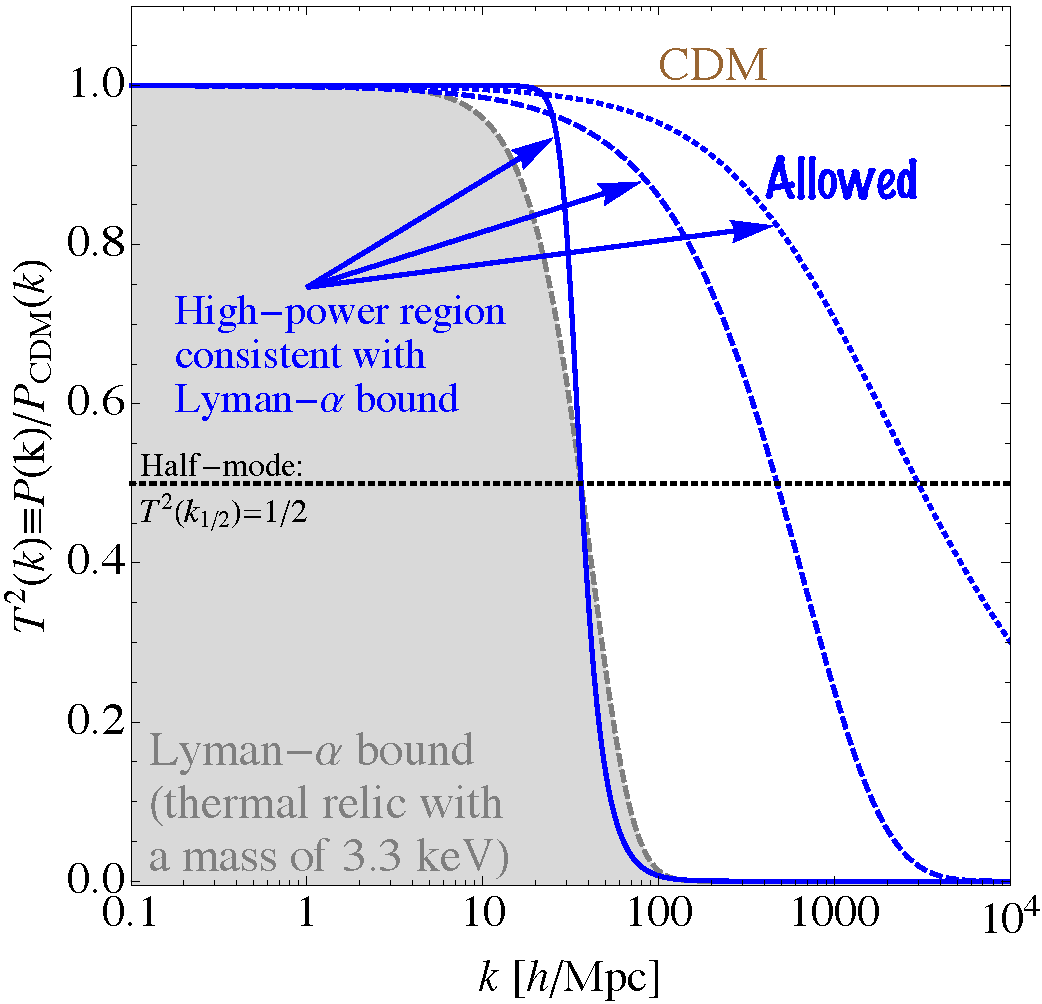
\includegraphics[width=8.3cm]{figures/DM_Allowed.pdf} & 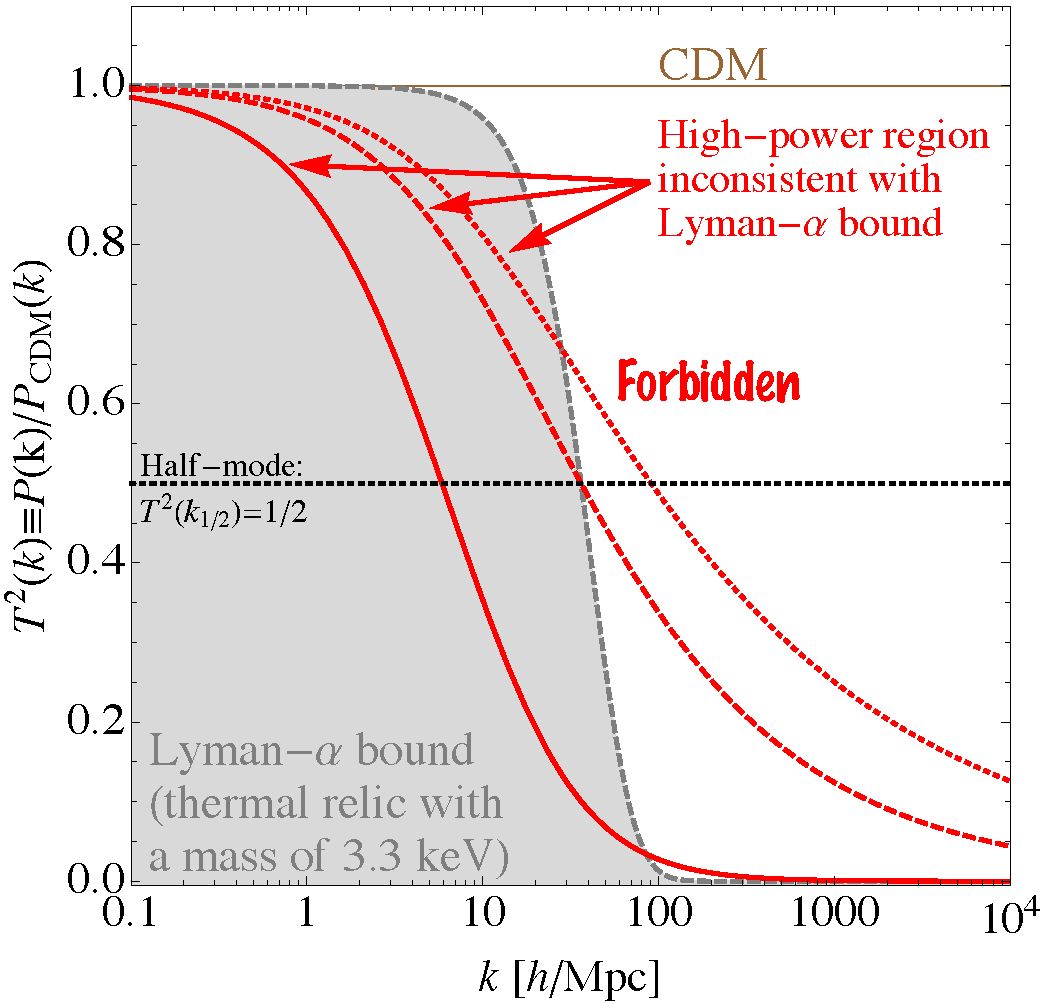
\includegraphics[width=8.3cm]{figures/DM_Forbidden.pdf}
\end{tabular}
\caption{\label{fig:Ly-alpha_illustration}Illustration of how we classify certain squared transfer functions as consistent (\emph{left}) or inconsistent (\emph{right}) with a certain bound.}
\end{figure}

There is a problem with this procedure, though. In some cases, $\mathcal{T}^2\left(k\right) \geq \sub{\mathcal{T}^2}{lim}\left(k\right)$ might only hold true for a certain interval of wave numbers $k$, but not for the  entire range. For example, $\mathcal{T}^2\left(k\right) \geq \sub{\mathcal{T}^2}{lim}\left(k\right)$ could be true for all $k$ smaller than a particular value $\tilde k$, but not anymore for $k > \tilde k$. This complication originates from the very fact that the limiting transfer functions are derived from thermal spectra, while realistic spectra can be highly non-thermal, which results in a difference in the exact evolution of the squared transfer function around its cutoff (e.g., the slope may be different).

In order to still use the limiting squared transfer functions, which are very good estimators accounting for observational relevance, we have developed the following procedure:
\begin{enumerate}

\item First, we compute the half-mode $k_{1/2}$, i.e., the wave number at which the squared transfer function has dropped to $1/2$:
\begin{align}
 k_{1/2}\ :\Longleftrightarrow\ \mathcal{T}^2\left(k_{1/2}\right) \stackrel{!}{=} 1/2 \;.
 \label{eq:Def:Half-mode}
\end{align}

\item Subsequently, we check whether $\mathcal{T}^2\left(k\right) \geq \sub{\mathcal{T}^2}{lim}\left(k\right)$ is fulfilled all $k \leq k_{1/2}$. If the condition is met within this range of small wave numbers (i.e., larger length scales), we consider the model as being consistent with a given bound. This is clearly an approximate method, since we intrinsically disregard some relevant information (namely the power spectrum below the half-mode). Furthermore, the value of $1/2$ is, ultimately, pure choice and one could equally well justify other values. However, it is clear that the border has to be somewhere between the two extreme cases of a certain squared transfer functions being completely untouched by the Lyman-$\alpha$ bounds (restrictive view) or by at least in small parts being allowed by the bound (conservation view), which is why a value of $1/2$ appears to be a fair compromise. We have in addition shown that our results are, in fact, quite robust with respect to this arbitrary choice: due to the power spectra considered still having a slope somewhat similar to that of a thermal relic, even a choice of $0.05$ instead of $0.5$ would not alter our results very significantly, cf.\ App.~\ref{app:D:HalfmodeThreshold}. We are currently working on more advanced analyses that will result into even more reliable procedures.

\end{enumerate}
This procedure is in fact rather simple, as can be seen from the cartoon-like illustration in Fig.~\ref{fig:Ly-alpha_illustration}. For the Lyman-$\alpha$ bounds, we use the squared transfer functions derived from thermal spectra with thermal masses of $m_{\rm lim} = \unit{2.0}{keV}$ ($m_{\rm lim} = \unit{3.3}{keV}$) in a conservative (more restrictive) scenario. Note that only the restrictive bound is displayed in Fig.~\ref{fig:Ly-alpha_illustration}, as the purpose of this figure is only to illustrate the principles behind the procedure, while later on we will display both bounds for completeness. The values quoted are motivated in~\cite{Viel:2005qj}, where the authors also provide an analytical fit formula for the transfer function of a given thermally distributed species of mass $m_{\rm lim}$, which is assumed to make up all the DM.

\paragraph{Bounds from the observed amount of dark radiation}
The combination of the momentum distribution function of the sterile neutrino and its mass is also constrained by the observation of the cosmic microwave background (CMB) and by the light element abundances related to big bang nucleosynthesis (BBN). The corresponding observables allow to constrain the effective number $\sub{N}{eff}$ of neutrinos and its deviation from the SM value of $3.046$~\cite{Mangano:2005cc}. The effective number of neutrinos is a measure of the radiation present in anything else than photons at a given epoch. It is therefore a measure of the Universe's expansion rate, which in turn leaves its imprint on both the CMB and the abundances of the elements produced during BBN. A similar analysis was shown in \cite[fig.~9]{Merle:2015oja}, however, with a small error in the numerical computation of the contribution to $\Delta\sub{N}{eff}$ from the non-cold sterile neutrinos. While this error led to an overestimation of their impact, these bounds would in any case only be relevant in the region that is already excluded by the requirement of DM not being classified as ``hot''. Of course the precise numbers have to be computed numerically, but it can easily be understood that the bounds from structure formation and from $\sub{N}{eff}$ must be closely related, since they both critically depend on how long DM stays ultra-relativistic.
  
Note that, apart from possibly impacting the region in the parameter space where the DM is produced extremely late, the dark radiation bound could in fact also be relevant for very small DM masses. However, as we have seen, any value of $m_N$ below $0.5$~keV is already excluded by the TG bound.


\paragraph{Model-dependent bounds on the most minimal particle physics setting}
So far, we have fixed the mass of the sterile neutrino by matching its number density to the observed DM energy density. In the most minimal setting, we could simultaneously demand that the mass of the sterile neutrino is generated by a VEV of the singlet scalar $S$, i.e., $m_N=y\av{S}$. This would allow us to use bounds from perturbative unitarity and bounds derived on the scalar mixing angle from its contribution to the $W$-mass. In principle, there are also direct collider bounds~\cite{Robens:2015gla}, but they are off our plots and do in practice not constrain the relevant region of the parameter space.

Following~\cite{Robens:2015gla}, we can bound the VEV of the scalar by:
\begin{align}
 \av{S} \geq \sqrt{\frac{3}{16 \pi}} m_S.
 \label{eq:PerturbativeUnitarity}
\end{align}
Using $\av{S} = \frac{m_N}{y}$ enables us to conclude an upper bound on the Yukawa coupling:
\begin{align}
 y \leq \frac{m_N}{m_S} \sqrt{\frac{16\pi}{3}} \,.
 \label{eq:PerturbativeUnitarity2}
\end{align}

A singlet scalar mixing with the Higgs via its VEV can also yield a radiative correction to the $W$-boson mass. Combining Eqs.~(8), (9), and~(11) from Ref.~\cite{Robens:2015gla}, we can deduce an upper limit on the Higgs portal coupling:
\begin{align}
 \lambda \leq \lambda^{\mathrm{max}} = y \sin^{\mathrm{max}}\left(2\alpha\right) \frac{|m_S^2 -m_h^2|}{2\sub{v}{EW} m_N} \,,
 \label{eq:W-mass-bound}
\end{align}
where $\sub{v}{EW}$ is the VEV of the SM-Higgs and $\alpha$ is related to the mixing of the scalars.\\

This completes our list of bounds which can possibly be relevant. As we will see, apart from the Lyman-$\alpha$ bound, the most relevant constraint arises from the TG bound. In the most minimal setting, collider-related constraints can become relevant, too, however these are strongly model-dependent and in fact very easy to circumvent. Finally, the overclosure and dark radiation bounds play no role in practice.



%%%%%%%%%%%%%%%%%%%%%%%%%%%%%%%%%%%%%%%%%%%%%%%%%%%%%%%%%%